\chapter{Beacon}
\label{chap:beacon}
Un beacon è una piccola antenna trasmettitore
bluetooth, che lavora alla frequenza standard di 2,4 ghz (la stessa del Wi-fi, per intendersi). Un beacon può inviare soltanto una piccola stringa di
codice, grande qualche manciata di byte, che funge da identificatore del
beacon stesso.

Nel corso degli anni le tipologie di beacon sono aumentate col trascorrere del tempo. Ad oggi, le tre principali tipologie di beacon sono:
\begin{enumerate}
\item iBeacon\index{iBeacon} - Apple
\item EddyStone - Google
\item AltBeacon - Open
\end{enumerate}

Il prodotto della Apple è stato il primo ad entrare nel mercato e per questo è il più diffuso in commercio.
Degli iBeacon verrà fatta una panoramica più ampia nel prossimo paragrafo, per il momento diciamo soltanto che prevede un solo tipo di frame.
EddyStone è un prodotto Google che funziona sia con Android che con iOS. La principale differenza rispetto al prodotto Apple, è la possibilità di scegliere tra due diversi tipi frame da inviare in broadcast. Per finire, AltBeacon nasce con l'esigenza di creare un protocollo per i beacon che sia aperto e che faccia dell'interoperabilità il suo punto di forza.
\section{iBeacon}
iBeacon technology\cite{apple}, introdotta con iOS7, è una tecnologia che permette di migliorare la localizzazione per app.
Utilizzando il Bluetooth Low Energy (BLE), un device che supporta gli iBeacon può essere utilizzato per stabilire se esso è dentro la regione di un determinato oggetto. 
Quindi, Permette ad un dispositivo iOS di determinare quando quest'ultimo entra o esce da una regione, con una stima della prossimità dal beacon.

Se si è interessati ad utilizzare gli ibeacon, si rientra in almeno una delle seguenti categorie di persone:
\begin{enumerate}
\item \textbf{App Developers}
\\Se si vuole migliorare la geo-localizzazione di un'app, si può utilizzare il Core Location APIs in iOS per ricevere notifiche quando un dispositivo entra ed esce dalla regione di un beacon e per stimare la prossimità dal beacon stesso. 
Tutto quello di cui si ha bisogno è incluso in iOS SDK.
\item \textbf{Persone che vogliono utilizzare un dispositivo con la tecnologia iBeacon}
\\Se si è interessati ad utilizzare il logo di iBeacon, ma non si è un produttore di iBeacon, si deve ottenere una licenza del logo prima di utilizzarlo.
\url{https://developer.apple.com/ibeacon/}   
\item \textbf{Persone che vogliono creare dispositivi con la tecnologia iBeacon}
\\Se si è interessati a costruire dispositivi con iBeacon technology, si deve ottenere una licenza da Apple prima di realizzarli. 
Con la licenza si ha l'accesso a specifiche tecniche  ed il permesso ad utilizzare il logo iBeacon. 
\end{enumerate}

Passiamo ora a descrive il frame.
Un iBeacon advertisement invia le seguenti informazioni via BLE:
\begin{table}[htbp]
\begin{center}
\begin{tabular}{|l|l|l|}
\hline
Campo & Dimensione & Descrizione \\
\hline
UUID & 16 bytes & Lo sviluppatore dovrebbe definirne uno\\
& & per la propria app e utilizzo \\
\hline
Major & 2 bytes & Indica uno specifico caso d'uso dell'iBeacon\\
\hline
Minor & 2 bytes & Suddivide ulteriormente la regione\\
\hline
\end{tabular}
\end{center}
\caption{iBeacon advertisement}
\label{tab:ibeacon}
\end{table}
\\UUID, major e minor identificano unicamente il beacon. 
Un UUID può essere generato utilizzando il comando \texttt{uuidgen} da terminale in OS X, o tramite  la classe NSUUID.
La seguente tabella mostra come questi valori possano essere utilizzati da una catena di negozi. 
\begin{table}[htbp]
\begin{center}
\begin{tabular}{|c|c|c|c|}
\hline
Negozio & Ancona & Jesi & Camerino \\
\hline
UUID &
\multicolumn{3}{c|}{D9B9EC1F-3925-43D0-80A9-1E39D4CEA95C} \\
\hline
Major & 1 & 2 & 3\\
\hline
Minor - Vestiti  & 10 & 10 & 10\\
\hline
Minor - Scarpe & 20 & 20 & 20\\
\hline
Minor - Intimo & 30 & 30 & 30\\
\hline
\end{tabular}
\end{center}
\caption{Esempio utilizzo UUID, major e minor}
\label{tab:example}
\end{table}
Utilizzando queste informazioni, un dispositivo iOS può identificare quando entra ed esce da un negozio e in che tipologia di negozio si trova. 
\\
iBeacon utilizzano il BLE, perciò richiede un iPhone 4s(o superiori), iPod touch(quinta generazione), iPad(terza generazione o iPad mini).
\subsection{Privacy and Location}
Dato che la tecnologia iBeacon è parte del Core Location, le stesse autorizzazioni sono richieste per poter essere utilizzata(vedi Figura \ref{fig:autorizzazioni}).
L'utente visualizzerà lo stesso alert quando un'applicazione tenterà di utilizzare le API di iBeacon\footnote{NOTA: Ciascun pacchetto Bluetooth che è associato con gli iBeacon sarà escluso dalle API del CoreBluetooth, nonostante ciò, senza attivare il Bluetooth le API di iBeacon non funzioneranno.}.
\begin{figure}[t]
\centering
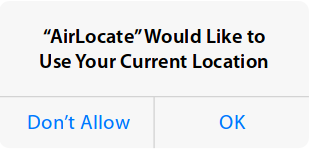
\includegraphics[scale=0.6]{Immagini/alert.png}
\caption{Autorizzazioni iOS} 
\label{fig:autorizzazioni}
\end{figure}\\
Come quando è attivo il GPS, quando utilizziamo la tecnologia iBeacon sarà presente una freccia nella status bar.
\subsection{Precisione degli iBeacon}
Per migliorare la user experience, è importante prendere in considerazione come il segnale dei beacon viene letto e utilizzato per determinare la distanza da esso. 
Quando un dispositivo iOS rileva un beacon, utilizza la potenza del segnale (RSSI - Received Signal Strength Indication)\index{RSSI} per determinare la proximity dal beacon.
Più potente è il segnale e migliore sarà la stima fatta dal device.
La potenza del segnale ricevuta è generalmente correlata dalla distanza fra il beacon e il dispositivo. 
In una condizione ideale la vicinanza del dispositivo dal beacon migliora la precisione.
Quando un dispositivo è lontano dal beacon, la potenza del segnale sarà minore rispetto a quando è vicino. 
Minore è la potenza del segnale, minore sarà la precisione nel calcolo della prossimità. 
Ad esempio, se ci troviamo a un metro di distanza il segnale sarà forte e la distanza dal dispositivo sarà calcolata con un errore di qualche cm.
Altrimenti, se ci troviamo a dieci metri di distanza il segnale sarà debole e la distanza dal dispositivo sarà calcolata con l'errore di qualche metro. 
Come per il segnale GPS, anche quello del beacon può essere ostacolato da un oggetto fisico.  
Il corpo umano, per esempio, può attenuare il segnale Bluetooth. 
Basta dare le spalle al beacon per diminuire la precisione del dispositivo nel calcolare la distanza dal beacon.

Quando si costruisce un'applicazione che utilizza GPS o beacon, è importante prendere in considerazione la precisione.
Il valore riportato dall'oggetto Core Location, indica il livello di incertezza, o margine di errore misurato in metri. 

\subsection{Monitoraggio regioni}
In maniera simile al monitoraggio di regioni con geofence, un'applicazione può richiedere di ricevere una notifica quando un dispositivo entra o lascia una regione definita da un beacon. 
Quando si crea la richiesta si deve specificare l'UUID dell'iBeacon advertisement. Mentre un'applicazione può monitorare un numero limitato di 20 regioni, usando un singolo UUID in più zone, un dispositivo può monitorare svariate zone contemporaneamente.

In aggiunta all'UUID, un applicazione può selezionare il major ed il minor per rendere più specifica la regione da monitorare.

Come per il monitoraggio di regioni con il GPS, quando un utente entra o esce da una regione l'applicazione riceverà una notifica. 
Se l'applicazione non è in esecuzione(per esempio se è stata terminate per necessità di ram da parte del sistema), l'applicazione verrà lanciata in background e gli verrà inoltrata la notifica. 
Un'importante considerazione sta nel fatto che se l'utente disabilita "Background App Refresh" allora l'app non verrà riavviata e quindi non riceverà le notifiche.

\subsection{Ranging}
iOS 7 ha introdotto un nuovo set di API per determinare approssimativamente la prossimità utilizzando iBeacon technology, processo conosciuto come "Ranging". 
Basandosi sui più comuni scenari, iOS applica dei filtri alla precisione calcolata per determinare una stima della prossimità dal beacon.
Questa stima è indicata utilizzando uno dei seguenti stati di prossimità:
\begin{table}[htbp]
\begin{center}
\begin{tabular}{|l|p{9cm}|}
\hline
Proximity State & Descrizione \\
\hline
Immediate & Indica l'immediata vicinanza del dispositivo al beacon \\
\hline
Near & Se non ci sono ostacoli tra il beacon ed il dispositivo, indica una distanza approssimativa che va da 1 a 3 metri. \\
\hline
Far & Questo stato indica che un beacon è stato rilevato ma non si è in grado di determinare se si è Near o Immediate. 
Un'importante considerazione è che questo stato non implica che si è lontani dal beacon.\\
\hline
Unknow & La prossimità dal beacon non può essere determinato.
Questo può indicare che il ranging è appena iniziato. \\
\hline
\end{tabular}
\end{center}
\caption{Proximity state}
\label{tab:state}
\end{table}

\subsection{Physical limitations}
I dispositivi iBeacon utilizzano il Bluetooth Low Energy\index{BLE} per inviare i messaggi.
BLE lavora ad una frequenza di 2.4GHz e può essere soggetto ad attenuazioni da qualsiasi oggetto fisico come pareti, porte o qualsiasi altro oggetto. La frequenza 2,4 GHz può essere ostacolata anche dall'acqua, ciò significa che anche le persone attenuano il segnale. Come detto precedentemente, quando il segnale ricevuto è debole, diminuisce la capacità del dispositivo di calcolare una stima della prossimità.
\subsection{Calibrazione}
Per migliorare la user experience, un aspetto fondamentale è la calibrazione dei beacon nel vostro sistema.
È consigliato eseguirla per ogni singolo dispositivo.
Il calcolo della distanza da parte del Core Location è effettuato utilizzando il valore Measured Power ottenuto, appunto, con la calibrazione. 
Per eseguirla dobbiamo:
\begin{enumerate}
\item Installare il beacon;
\item Utilizzando un dispositivo con iOS 7 o superiore con il Bluetooth 4.0, campionare la potenza del segnale ad un metro di distanza per un minimo di 10 secondi. In questa fase bisogna ricordarsi di tenere il dispositivo  in verticale e di lasciare libera la metà superiore del device.
\item Muovere il dispositivo avanti e indietro lentamente per 30cm mantenendo l'orientamento e la distanza dal beacon(vedi Figura \ref{fig:calibrazione}). 
\begin{figure}[htbp]
\centering
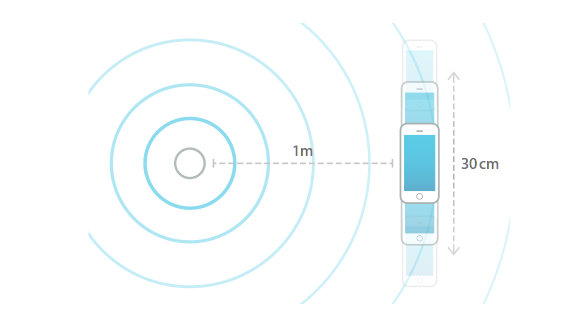
\includegraphics[scale=0.6]{Immagini/fig5.png}
\caption{Calibrazione} 
\label{fig:calibrazione}
\end{figure}\\
\item Calcolare la media dei valori \textit{rssi} registrati per ottenere la \textbf{Measured Power};
\item Applicare il valore di \textbf{Measured Power} al beacon;
\end{enumerate}
Dato che il sistema circostante può influire sulla frequenza del bluetooth, è importante ripetere la procedura per ogni beacon installato. 
\subsection{UUID}
Un \textbf{Universally Unique IDentifier}(UUID)\index{UUID} definito in RFC 4122\cite{RFC4122} è un identificatore standard usato per la costruzione di applicazioni.
Esso è semplicemente un numero rappresentato da 128 bit.
Il significato di ogni bit è definito nella specifica di ciascuna delle sue varianti.

Per essere letti anche dagli esseri umani, molti sistemi lo rappresentano in esadecimale inserendo dei caratteri dash al suo interno. Un esempio:
\textbf{de305d54-75b4-431b-adb2-eb6b9e546014} 

L'obiettivo degli UUID è quello di distribuire sistemi con un id univoco senza un'unità centrale di controllo. In questo contesto la parola univoco prende il significato di "praticamente univoco" e non garantisce niente. 
Chiunque può creare un UUID ed utilizzarlo per identificare qualcosa sapendo che le probabilità che qualcun altro generi lo stesso UUID sono veramente basse, se non nulle.

Un UUID è formattato secondo le specifiche delle varianti.
Esistono 5 varianti di UUID:
\begin{enumerate}
\item Version 1 (MAC address \& data-time)
\item Version 2 (DCE Security);
\item Version 3 (MD5 hash \& namespace);
\item Version 4 (random);
\item Version 5 (SHA-1 hash \& namespace).
\end{enumerate}

Se ai 128 bit togliamo i due bit che identificano RFC 4122 e i 4 che identificano la versione, abbiamo che gli UUID generati hanno 122 bit random.
La possibilità che due UUID abbiamo lo stesso identico valore può essere calcolata utilizzando il calcolo della  probabilità (il problema del compleanno).
\begin{equation}
p(n)\cong1-e^{-\frac{n^2}{2-2^x}}
\end{equation}
Questa è la probabilità di una collisione calcolando $n$ UUID, con $x = 122$:
\begin{table}[htbp]
\begin{center}
\begin{tabular}{|c|c|}
\hline
n & probabilità\\
\hline
$65.719.476.736 = 2^{36}$ & $0,0000000000000004 = 4( 10^{-16})$\\
\hline
$2.199.023.255.552 = 2^{41}$ & $0,0000000000005 = 5( 10^{-13})$\\
\hline
$70.368.744.177.664 = 2^{46}$ & $0,0000000005 = 5( 10^{-10})$\\
\hline
\end{tabular}
\end{center}
\caption{Probababilità collisione UUID}
\label{tab:collisione}
\end{table}

\section{BlueUp}
Tra le diverse aziende presenti nel mercato, abbiamo scelto un'azienda italiana per l'acquisto dei nostri primi beacon: la BlueUp.
\subsection{BlueBeacon}
BlueUp realizza beacon e sensori con tecnologia Bluetooth Low Energy: la serie BlueBeacon\footnote{Per maggiori informazioni riguardo le caratteristiche tecniche dei prodotti BlueUp si rimanda alla bibliografia\cite{blueup}}\index{BlueBeacon} offre una delle più ampie selezioni del mercato. 

I dispositivi BlueBeacon sono proposti in due versioni firmware, che supportano i principali standard presenti sul mercato: 
la tecnologia iBeacon di Apple oppure la specifica Eddystone di Google.
\subsection{Caratteristiche}
I BlueBeacon hanno prestazioni radio ottime, superiori alla maggior parte dei dispositivi beacon in commercio. 
Questo risultato è garantito da una serie di scelte tecnologiche che sono state adottate sui BlueBeacon:
\begin{itemize}
\item utilizzo del chip radio Nordic nRF51822, che garantisce ottime prestazioni a livello radio e di consumi;
\item antenna stampata su PCB di tipo meandered PIFA (Planar Inverted F Antenna) che offre prestazioni superiori in termini di guadagno rispetto alle antenne a chip comunemente adottate;
\item antenna progettata per essere adattata in presenza dell'involucro plastico, riducendo quindi le perdite per riflessione;
\item rete di adattamento RF basata su singolo chip (balun), che riduce le perdite di inserzione rispetto alle convenzionali reti ad elementi discreti;
\end{itemize}

Grazie a queste soluzioni, i BlueBeacon, a parità di potenza emessa dal chip radio, trasmettono un livello di potenza superiore di un fattore 2 - 4 rispetto ad altri dispositivi. 
Questo permette di ridurre la potenza emessa dal chip, con un conseguente riduzione dei consumi e, quindi, aumento della vita operativa delle batterie. 
Inoltre, un segnale con un livello di potenza maggiore garantisce una superiore stabilità in ricezione e un aumento della distanza di comunicazione del beacon. 
\subsection{Trasmissione}
La misura della distanza con i beacon è basata sul valore dell'RSSI (Received Signal Strength Indicator), ovvero della potenza del segnale RF ricevuto dallo smartphone. 
Il segnale ricevuto risente fortemente di una serie di elementi, fra cui, l'orientazione e la posizione relative dello smartphone rispetto al beacon, la presenza del corpo umano, fenomeni di riflessione e diffrazione dall'ambiente (soprattutto struttire metalliche).
Di conseguenza, il valore di RSSI non può fornire una misura esatta della distanza in un ambiente complesso (questa condizione sarebbe vera solo nel caso ideale di spazio libero), ma solo una stima approssimata della vicinanza dello smartphone dal beacon. 
Da tenere in conto, inoltre, che l'accuratezza è fortemente dipendente dall'intervallo di advertising. 

La massima distanza di trasmissione (ovvero la massima distanza a cui può essere ricevuto il segnale trasmesso dal beacon) dipende da una serie di parametri. 
Il più importante è la potenza trasmessa: maggiore è la potenza trasmessa è maggiore è la distanza, anche se non c'è una relazione di linearità fra le due grandezze, a causa dei meccanismi fisici di propagazione. 
Altri aspetti che hanno un impatto sulla distanza di trasmissione sono:
\begin{itemize}
\item il punto di installazione del beacon: più il beacon è posto in alto, maggiore è la distanza di comunicazione
\item l'ambiente operativo: la presenza di ostacoli, oggetti (soprattutto metalli e liquidi), persone, frapposti (o in prossimità) fra il beacon ed il ricevitore ha un impatto non trascurabile sulla distanza
\item le prestazioni del ricevitore: la sensibilità e il guadagno del ricevitore variano da modello a modello di smartphone, e inoltre la sensibilità può essere anche affetta da fattori esterni, come la presenza di altri dispositivi radio
\item altri fattori, fra cui l'orientazione reciproca fra beacon e smartphone, il modo come viene impugnato lo smartphone da parte dell'utente.
\end{itemize}

La tabella \ref{tab:distanza}, riporta la distanza massima teorica, nel caso di diversi valori di potenza trasmessa, valutata nell'ipotesi di un ricevitore (smartphone) con sensibilità (minimo valore di RSSI ricevibile) pari a -90dBm. 
I risultati della tabella sono stimati nel caso di beacon e smartphone posti a 1.5 metri di altezza, in linea di vista, in spazio libero.
\begin{table}[htbp]
\begin{center}
\begin{tabular}{|c|c|c|c|c|}
\hline
 & Mini & Maxi & Forte & USB\\
\hline
\textbf{+4 dBm} & 100m & 100m & 110m & -\\
\hline
\textbf{+0 dBm} & 60m & 60m & 65m & 30m\\
\hline
\textbf{-8 dBm} & 25m & 25m & 30m & 12m\\
\hline
\textbf{-20 dBm} & 6m & 6m & 7m & 3m\\
\hline
\end{tabular}
\end{center}
\caption{Distanza massima di trasmissione}
\label{tab:distanza}
\end{table}
\subsection{Batteria}
La vita operativa della batteria del BlueBeacon dipende da un serie di fattori: 
intervallo di advertising (fattore principale), potenza trasmessa, valore e variazioni della temperatura operativa, modalità operativa ("non-connectable mode" o "connectable mode"). 
La tabella \ref{tab:batteria} riporta la vita operativa attesa (in mesi, espressa in funzione della potenza trasmessa e dell'intervallo di advertising), per ognuno dei beacon a batteria, BlueBeacon Mini, Maxi e Forte. 
I valori sono stimati sulla base delle misure di laboratorio di assorbimento di corrente e dei valori nominali di capacità e autoscarica forniti dal produttore della batteria. 
La temperatura operativa è ipotizzata di circa 20C: nel caso di valori di temperatura estremi (in particolare molto bassi), la vita operativa può essere limitata. 
Le misure sono effettuate con i beacon configurati in "non-connectable mode". Se i beacon sono in "connectable mode", la vita operativa della batteria si può ridurre fino al 30\% in meno.
\begin{table}[htbp]
\begin{center}
\begin{tabular}{|c|c|c|c|c|c|}
\hline
 & 0,1 sec & 0,3 sec & 0,5 sec & 0,7 sec & 1,0 sec\\
\hline
\textbf{+0 dBm} & 4 & 11 & 16 & 20 & 25\\
\hline
\textbf{-8 dBm} & 4,5 & 11,5 & 17 & 22 & 27\\
\hline
\textbf{-20 dBm} & 5 & 12,5 & 19 & 24 & 29\\
\hline
\end{tabular}
\end{center}
\caption{Durata batteria BlueBeacon Mini in mesi}
\label{tab:batteria}
\end{table}

\section{Utilizzo dei Beacon in Proximity System}
Inizialmente si era pensato di realizzare un prodotto che eseguisse operazioni sull'ufficio basandosi unicamente sulla posizione dell'utente all'interno di esso, da qui il nome Proximity System.
In seguito, abbiamo stabilito che, nonostante l'esecuzione automatica di determinate azioni a seconda della posizione doveva rimanere la caratteristiche principale, il tutto deve poter funzionare anche senza beacon.
Per questo motivo, abbiamo previsto tre modalità di funzionamento per i singoli dispositivi:
\begin{enumerate}
\item \textbf{Manuale}: l'utente può comandare il dispositivo da qualsiasi posizione;
\item \textbf{Semi-automatica}: l'utente può comandare il dispositivo solo se si trova all'interno della regione del beacon associato al dispositivo; 
\item \textbf{Automatica}: il dispositivo si accende e spegne automaticamente rispettivamente se un un utente entra o esce dalla regione del beacon associato.
\end{enumerate}